\documentclass[11pt,a4paper]{article}

\usepackage[margin=2.3cm]{geometry}
\usepackage{amsmath,amssymb}
\usepackage{booktabs}
\usepackage{array}
\usepackage{graphicx}
\usepackage{float}
\usepackage[hidelinks]{hyperref}

\newcommand{\eps}{\varepsilon}
\newcommand{\dd}{\mathrm{d}}
\newcommand{\jj}{\mathrm{j}}
\newcommand{\Erms}{E_{\mathrm{rms}}}
\usepackage{xurl}
\DeclareUrlCommand\code{\urlstyle{tt}}

\title{The mathematics behind \texttt{insulated\_monopole\_Erms.m}\\[4pt]
\large Time-RMS electric field in a Phytagel phantom below an insulated\\ 2.45\,GHz monopole in water}
\author{BMET3921 -- microwave catheter heating project}
\date{28 September 2026}

\begin{document}
\maketitle

\section{Purpose and overview}

The script \code{V5_convection/Insulated_monopole_Erms/insulated_monopole_Erms.m} computes the
time-RMS electric field $\Erms$ in the vertical plane of the gel phantom that lies directly under a
2.45\,GHz monopole. The antenna lies horizontally in circulating water just above the gel surface. The field
map is the source term for the dielectric heating of the gel ($Q=\sigma_{\text{eff}}\Erms^2$). It was built to
reproduce the photographed run (50\,W generator setting, continuous wave, 6 minutes), in which the heated
region in the gel peaks about 3\,mm \emph{in front of} the feed point instead of directly beneath it.

The earlier cylindrical master formula (\code{Dielectric_heating/cylindrical_master_formula.m}) assumed
a uniform cylindrical power flow $P/(2\pi r L)$. That form has no dependence on position along the antenna,
so it cannot place a hot spot anywhere along the element. The model described here replaces it with a
physical current distribution. The calculation has four stages, and each is derived below:
\begin{enumerate}
  \item the complex wavenumber $k_L$ of the current travelling along an \emph{insulated} conductor
        immersed in water, from King's insulated-antenna theory;
  \item the input impedance of the element, and from it the feed current $I_0$ that delivers the
        measured power;
  \item the current $I(x')$ and line charge $q(x')$ along the element and the exposed feed block;
  \item the electric field these sources produce in the gel, from the retarded potentials, with a
        correction for the water--gel interface.
\end{enumerate}
Section~\ref{sec:constants} lists every input number with its source. Assumptions are stated where
they enter the derivation and collected in Section~\ref{sec:assumptions}.

\section{Conventions}\label{sec:conventions}

All fields are time-harmonic, and the script uses the engineering convention
\begin{equation}
  \mathbf{E}(\mathbf{r},t) = \operatorname{Re}\!\left\{\mathbf{E}(\mathbf{r})\,e^{\jj\omega t}\right\},
  \qquad \omega = 2\pi f,\quad f = 2.45\ \text{GHz},
\end{equation}
where the phasor $\mathbf{E}(\mathbf{r})$ holds the \emph{peak} amplitude. With this convention a lossy
medium has the complex relative permittivity
\begin{equation}
  \eps_r = \eps' - \jj\eps'', \qquad \sigma_{\text{eff}} = \omega\eps_0\eps'',
  \label{eq:complexeps}
\end{equation}
so that all conduction and dielectric loss appear in $\eps''$ \cite{Harrington1961}. The wavenumber in
each medium is
\begin{equation}
  k = k_0\sqrt{\eps_r}, \qquad k_0 = \frac{\omega}{c_0} = 51.35\ \text{rad/m},
  \label{eq:k}
\end{equation}
taking the root with $\operatorname{Im}k<0$ so that an outgoing wave $e^{-\jj kR}$ decays. For the three
media this gives
\begin{gather*}
  k_{\text{ins}} = 74.41\ \text{rad/m (PTFE)},\qquad
  k_w = 439.5-26.4\jj\ \text{rad/m (water)},\\
  k_g = 344.4-51.7\jj\ \text{rad/m (gel)}.
\end{gather*}
In the gel the wavelength is $2\pi/\operatorname{Re}k_g = 18.2$\,mm and the field $1/e$ decay length is
$1/|\operatorname{Im}k_g| = 19.4$\,mm. Both are larger than the 10\,mm deep region that is mapped. The field
is therefore neither purely quasi-static nor strongly attenuated, and the full retarded Green's function is
kept in Section~\ref{sec:field}.

King and co-workers \cite{King1983,KingSmith1981} use the physics convention $e^{-i\omega t}$. Their formulas
are converted here by the substitutions $i\to-\jj$ and $H^{(1)}_n\to H^{(2)}_n$, where the Hankel function
of the second kind represents an outgoing wave under $e^{\jj\omega t}$.

\section{Experimental constants}\label{sec:constants}

Table~\ref{tab:constants} lists the inputs. Values labelled ``setup table'' come from
\code{V5_convection/Experimental_setup_table.xlsx}. The geometry was measured from the photograph
\code{Gel_model_V3/mirrored.jpg} at 105.8\,px/mm, because the photographed antenna is not the 27\,mm
antenna described in the setup table. Where the two sources differ, the table gives both values and marks
the one the script uses.

\begin{table}[tbp]
\centering
\caption{Constants used by \texttt{insulated\_monopole\_Erms.m}.}
\label{tab:constants}
\small
\begin{tabular}{>{\raggedright}p{4.6cm} c >{\raggedright}p{3.1cm} >{\raggedright\arraybackslash}p{5.2cm}}
\toprule
Quantity & Symbol & Value used & Source / remark \\
\midrule
\multicolumn{4}{l}{\emph{Excitation}}\\
Microwave frequency & $f$ & 2.45\,GHz & Setup table \\
Generator power setting & $P_{\text{set}}$ & 50\,W & Photographed run (the setup table's starting condition is 60\,W) \\
Reflected power & $P_{\text{refl}}$ & 0\,W & Setup table \\
Power dropoff (fraction lost before the antenna) & $P_{\text{dropoff}}$ & 0.7 & Setup table; a tunable estimate, so 30\% reaches the antenna \\
Delivered power & $P$ & 15\,W & $P_{\text{set}}(1-P_{\text{dropoff}})$ \\
\midrule
\multicolumn{4}{l}{\emph{Media}}\\
Gel relative permittivity, real & $\eps_g'$ & 43.98 & Setup table \\
Gel relative permittivity, imaginary & $\eps_g''$ & 13.5 & Setup table \\
Gel conductivity & $\sigma_g$ & (1.7\,S/m) & Setup table; not used directly. Eq.~\eqref{eq:complexeps} gives 1.84\,S/m from $\eps_g''$ \\
Water relative permittivity, real & $\eps_w'$ & 73 & Setup table \\
Water relative permittivity, imaginary & $\eps_w''$ & 8.8 & Setup table \\
Water temperature & $T_w$ & 37\,$^\circ$C & Setup table (context only) \\
Water flow, circulation / irrigation & -- & 5 / 0.03\,L/min & Setup table (context only; not used in the field model) \\
PTFE relative permittivity & $\eps_{\text{ins}}$ & 2.1 & Standard value for PTFE \cite{vonHippel1954}; loss neglected \\
\midrule
\multicolumn{4}{l}{\emph{Geometry}}\\
Element length, feed to tip & $L$ & 12\,mm & Photograph (the setup table's antenna is 27\,mm) \\
Inner conductor radius & $a$ & 0.15\,mm & RG-178 centre conductor, 0.30\,mm diameter \cite{MIL17} \\
PTFE insulation outer radius & $b$ & 0.42\,mm & RG-178 dielectric, $\approx$0.84\,mm diameter \cite{MIL17} \\
Exposed metal feed block & $l_f$ & 1.5\,mm & Photograph (solder/ferrule behind the feed) \\
Element axis above gel surface & $h$ & 1.1\,mm & Photograph (the setup table gives 2\,mm for the 27\,mm antenna) \\
Gel block height / length & -- & 30 / 30\,mm & Setup table; the model treats the gel as a half-space \\
\midrule
\multicolumn{4}{l}{\emph{Physical constants}}\\
Speed of light & $c_0$ & 299\,792\,458\,m/s & Exact (SI) \\
Permeability of free space & $\mu_0$ & $4\pi\times10^{-7}$\,H/m & \\
Permittivity of free space & $\eps_0$ & $8.854\times10^{-12}$\,F/m & \\
\bottomrule
\end{tabular}
\end{table}

The water values ($\eps'=73$, $\eps''=8.8$) are of the size predicted by the Debye relaxation of pure water
at 2.45\,GHz near body temperature \cite{Kaatze1989}. Treating the circulating water as pure water, with no
ionic conductivity, is an assumption. If the water is saline, $\eps_w''$ would be considerably larger.

\section{Stage 1: the current wavenumber on an insulated element}\label{sec:kL}

\subsection{Why a bare-wire wavenumber is wrong}

A bare conductor in water carries a current that varies along the wire roughly as $e^{\mp\jj k_w x}$, with
$k_w\approx 440$\,rad/m. The corresponding wavelength is about 14\,mm, so a 12\,mm element would be nearly a full
wavelength long. The element in the photographs, however, is the inner conductor of RG-178 with its PTFE
dielectric left on. The low-permittivity sleeve changes the current's propagation constant substantially.
King, Trembly and Strohbehn \cite{King1983}, following King and Smith \cite{KingSmith1981}, showed that the
insulated conductor behaves as a lossy transmission line whose ``outer conductor'' is the surrounding
medium.

\subsection{Transmission-line derivation}

Let the conductor of radius $a$ be covered by insulation of permittivity $\eps_{\text{ins}}$ out to radius
$b$, and be surrounded by water. The current $I(x)$ and the voltage $V(x)$ between the conductor and the
ambient medium obey the telegrapher's equations \cite{Pozar2012}
\begin{equation}
  \frac{\dd V}{\dd x} = -z\,I, \qquad \frac{\dd I}{\dd x} = -y\,V,
  \qquad\Rightarrow\qquad \frac{\dd^2 I}{\dd x^2} + k_L^2 I = 0,\quad k_L^2 = -zy,
  \label{eq:telegraph}
\end{equation}
where $z$ and $y$ are the series impedance and shunt admittance per unit length.

\paragraph{Shunt admittance.} The radial displacement current passes through the insulation and then the
water, which are in series. King's theory assumes \cite{King1983}
\begin{equation}
  \left|\frac{k_w}{k_{\text{ins}}}\right|^2 \gg 1 ,
  \label{eq:kingcond}
\end{equation}
Under this condition the admittance of the water path is so much larger than that of the insulation that
the insulation alone sets $y$:
\begin{equation}
  y = \jj\omega C', \qquad C' = \frac{2\pi\eps_0\eps_{\text{ins}}}{\ln(b/a)} = 113.5\ \text{pF/m}.
  \label{eq:C}
\end{equation}
Here $|k_w/k_{\text{ins}}|^2=35$, so the condition holds.

\paragraph{Series impedance.} The series impedance has two parts. The first is the magnetic flux inside the
insulation, identical to that of a coaxial line of radii $a$ and $b$. The second is the impedance of the
outgoing cylindrical TM wave set up in the water outside $\rho=b$. Its ratio $E_x/(2\pi b H_\phi)$ at the
insulation surface is a ratio of Hankel functions \cite{King1983,KingSmith1981}:
\begin{equation}
  z = \frac{\jj\omega\mu_0}{2\pi}\left[\ln\frac{b}{a} +
      \frac{H^{(2)}_0(k_w b)}{k_w b\,H^{(2)}_1(k_w b)}\right].
  \label{eq:z}
\end{equation}

\paragraph{Wavenumber.} Substituting \eqref{eq:C} and \eqref{eq:z} into $k_L^2=-zy$ and using
$\omega^2\mu_0\eps_0\eps_{\text{ins}}=k_{\text{ins}}^2$ gives
\begin{equation}
  \boxed{\,k_L = k_{\text{ins}}\left[1 + \frac{H^{(2)}_0(k_w b)}{k_w b\,H^{(2)}_1(k_w b)\,\ln(b/a)}\right]^{1/2}\,}
  \label{eq:kL}
\end{equation}
This is line 33 of the script. King's derivation also requires the insulation to be electrically thin,
$|k_{\text{ins}}b|^2\ll1$ (here $k_{\text{ins}}b=0.031$), and the outer radius to be small compared with the
wavelength in the ambient medium. Here $|k_w b|=0.185$, which satisfies the second condition.

\subsection{Physical interpretation}

Because $|k_wb|$ is small, the Hankel functions can be replaced by their small-argument forms
\cite{AbramowitzStegun1964}, $H^{(2)}_0(u)\approx1-\tfrac{2\jj}{\pi}\ln(\gamma' u/2)$ and
$uH^{(2)}_1(u)\approx \tfrac{2\jj}{\pi}$, with $\gamma'=e^{\gamma}\approx1.781$. The Hankel ratio then becomes
\begin{equation}
  \frac{H^{(2)}_0(k_w b)}{k_w b\,H^{(2)}_1(k_w b)} \approx \ln\frac{2}{\gamma' k_w b} - \jj\frac{\pi}{2},
\end{equation}
and the series impedance becomes
\begin{equation}
  z \approx \frac{\jj\omega\mu_0}{2\pi}\ln\frac{b_{\text{eff}}}{a} + \frac{\omega\mu_0}{4},
  \qquad b_{\text{eff}} = \frac{2}{\gamma' k_w},\quad |b_{\text{eff}}| \approx 2.6\ \text{mm}.
\end{equation}
The first term is the inductance of a coaxial line whose outer conductor is a shell of water about 2.6\,mm
from the axis. The second term is a real resistance, $\omega\mu_0/4\approx4.8$\,k$\Omega$/m, which accounts for
the power the line leaks into the lossy ambient medium. It is this term that makes $k_L$ complex. The
approximation gives $k_L\approx127.5-31.9\jj$\,rad/m, and the exact expression \eqref{eq:kL} evaluated by
the script gives
\begin{equation}
  k_L = 126.0 - 29.7\jj\ \text{rad/m},\qquad
  \lambda_L = \frac{2\pi}{\operatorname{Re}k_L} = 49.9\ \text{mm},\qquad
  \frac{\lambda_L}{4} = 12.5\ \text{mm}.
\end{equation}
The key result is that the 12\,mm insulated element is almost exactly a quarter wavelength of its own
current wave. The current is therefore largest at the feed and falls to zero at the tip, and it does not
oscillate along the element as a bare-wire model would predict.

\section{Stage 2: input impedance and feed current}\label{sec:feed}

\subsection{Input impedance}

The characteristic impedance of the line in \eqref{eq:telegraph} is
\begin{equation}
  Z_c = \sqrt{\frac{z}{y}} = \frac{\jj k_L}{y} = \frac{k_L}{\omega C'} = 72.2 - 17.0\jj\ \Omega .
\end{equation}
The tip is modelled as an open circuit, $I(L)=0$. This neglects the small fringing capacitance of the tip.
A section of line of length $L$ with an open end then has the input impedance \cite{Pozar2012}
\begin{equation}
  Z_{\text{in}} = Z_c\coth(\jj k_L L) = -\jj Z_c\cot(k_L L).
  \label{eq:Zin}
\end{equation}
With $k_LL = 1.512-0.356\jj$, this gives $Z_{\text{in}} = 23.9 - 9.6\jj\ \Omega$. The small reactance is
consistent with a line just shorter than $\lambda_L/4$.

Equation~\eqref{eq:Zin} treats the monopole as a \emph{single} open-circuited arm. In King's centre-fed
insulated dipole the two arms appear in series \cite{King1983}. Here there is only one arm, and the return
path is assumed to close through the feed block and the surrounding water (Section~\ref{sec:sources}). This is
a modelling assumption. It sets the absolute scale of $I_0$, but it has no effect on the \emph{shape} of the
field map.

\subsection{Feed current from the delivered power}

The time-average power entering a port of impedance $Z_{\text{in}}$ carrying a peak phasor current $I_0$ is
\cite{Pozar2012}
\begin{equation}
  P = \tfrac12\,|I_0|^2\operatorname{Re}Z_{\text{in}}
  \qquad\Rightarrow\qquad
  I_0 = \sqrt{\frac{2P}{\operatorname{Re}Z_{\text{in}}}} = 1.12\ \text{A},
  \label{eq:I0}
\end{equation}
with $P = P_{\text{set}}(1-P_{\text{dropoff}}) = 15$\,W. $I_0$ is taken to be real, which fixes the phase
reference. This step makes three assumptions:
\begin{itemize}
  \item all of $P$ is absorbed in the water and the gel, so ohmic loss in the conductor and dielectric loss
        in the PTFE are neglected;
  \item the reflected power is zero, as recorded in the setup table;
  \item the losses between the generator and the antenna are captured by the single factor
        $P_{\text{dropoff}}$, which is an estimate and not a measured value.
\end{itemize}
Because $\Erms\propto I_0\propto\sqrt{P}$, any error in $P_{\text{dropoff}}$ rescales the whole map without
moving the peak.

\section{Stage 3: current and charge on the antenna}\label{sec:sources}

\subsection{The element, $0<x'<L$}

Solving \eqref{eq:telegraph} with $I(0)=I_0$ and $I(L)=0$ gives King's standing-wave current
\cite{King1983,KingSmith1981}:
\begin{equation}
  I(x') = I_0\,\frac{\sin\!\big(k_L(L-x')\big)}{\sin(k_L L)}, \qquad 0<x'<L .
  \label{eq:Ielem}
\end{equation}
The feed is at $x'=0$ and the tip at $x'=L$. Because $k_L$ is complex, this sinusoid also decays slightly
along the element, with a $1/e$ length of $1/|\operatorname{Im}k_L|=34$\,mm.

The charge per unit length follows from the continuity equation
$\partial I/\partial x' + \jj\omega q = 0$ \cite{Jackson1999}:
\begin{equation}
  q(x') = \frac{\jj}{\omega}\frac{\dd I}{\dd x'}
        = -\frac{\jj k_L I_0}{\omega}\,\frac{\cos\!\big(k_L(L-x')\big)}{\sin(k_L L)}.
  \label{eq:qelem}
\end{equation}
Because the element is nearly a quarter wave long, $\cos(k_L L)$ is small. The charge is therefore
concentrated toward the tip: at the tip $|q|$ is 2.7 times its value at the feed.

\subsection{The feed block, $-l_f<x'<0$}

At the feed, current leaves the inner conductor and must return along the outside of the coax. The earlier
models placed this return on the braid. In V3 a 27\,mm braid arm carried the full current, which made the
source symmetric about the feed and put the heating peak directly under it, contrary to the photographs.
The present model assumes instead that there is \emph{no long sheath current}: the return current ramps
linearly to zero across the 1.5\,mm of exposed solder and ferrule behind the feed,
\begin{equation}
  I(x') = I_0\left(1+\frac{x'}{l_f}\right), \qquad
  q(x') = \frac{\jj}{\omega}\frac{\dd I}{\dd x'} = \frac{\jj I_0}{\omega l_f},
  \qquad -l_f<x'<0 .
  \label{eq:block}
\end{equation}
The linear profile is the simplest choice that is continuous with \eqref{eq:Ielem} at $x'=0$. It is an
assumption; the photographs do not resolve the actual distribution. The model is checked through total
charge. Integrating $q$ over both parts,
\begin{equation}
  \int_{-l_f}^{L} q\,\dd x' = \frac{\jj}{\omega}\Big[I(L) - I(-l_f)\Big] = 0 ,
\end{equation}
shows that the antenna is electrically neutral. The element carries total charge $-\jj I_0/\omega$, and the
feed block carries $+\jj I_0/\omega$ packed into only 1.5\,mm. The block's line-charge density is about 15
times that of the element next to the feed. This packed charge is the origin of the very strong field that
the model predicts at the gel surface just behind the feed (Section~\ref{sec:results}).

\section{Stage 4: the field in the gel}\label{sec:field}

\subsection{Retarded potentials}

The current and charge are treated as filaments on the antenna axis (the thin-wire approximation
\cite{Balanis2016}), which lies at height $h$ above the gel surface. In a homogeneous medium of wavenumber
$k$, the Lorenz-gauge potentials of an $x$-directed line source are \cite{Jackson1999,Balanis2016}
\begin{equation}
  \mathbf{A}(\mathbf r) = \hat{\mathbf x}\,\frac{\mu_0}{4\pi}\int I(x')\,G(R)\,\dd x', \qquad
  \phi(\mathbf r) = \frac{1}{4\pi\eps_0\eps_r}\int q(x')\,G(R)\,\dd x', \qquad
  G(R) = \frac{e^{-\jj kR}}{R},
  \label{eq:potentials}
\end{equation}
and the electric field is
\begin{equation}
  \mathbf E = -\jj\omega\mathbf A - \nabla\phi .
  \label{eq:EAphi}
\end{equation}
The script evaluates the field at points $(x,z)$ in the vertical plane that contains the antenna axis, with
$z=0$ at the gel surface and $z<0$ inside the gel. The distance from the axis is $\rho = h - z$, and the
distance to a source point is $R=\sqrt{(x-x')^2+\rho^2}$. Because the sources are axisymmetric, the only
field components are $E_x$ (along the antenna) and $E_\rho$ (radial, which is vertical in this plane).

The thin-wire approximation replaces the true sources, spread over radii up to $b=0.42$\,mm, by a filament
on the axis. The nearest field point is at $\rho=h=1.1$\,mm, about $2.6b$. The approximation is therefore
adequate in the gel but would not be valid at the insulation surface.

\subsection{The gradient of the Green's function}

$G$ depends only on $R$, so
\begin{equation}
  \frac{\dd G}{\dd R} = -\frac{(1+\jj kR)}{R}\,G, \qquad
  \frac{\partial R}{\partial x} = \frac{x-x'}{R}, \qquad
  \frac{\partial R}{\partial \rho} = \frac{\rho}{R}.
\end{equation}
The $1/R^2$ part of $\dd G/\dd R$ is the quasi-static (Coulomb) field of the charges. The $\jj k/R$ part is
their radiating contribution.

\subsection{The water--gel interface}

The sources lie in water ($\eps_w$), but the field is evaluated in the gel ($\eps_g$). The script uses the
gel Green's function, $k=k_g$ and $\eps_r=\eps_g$, and corrects the charge term with the quasi-static
transmission factor for a planar dielectric interface. Jackson \cite[\S4.4]{Jackson1999} shows that for a
point charge $q$ in medium 1 near a plane boundary with medium 2, the potential in medium 2 is that of a
charge
\begin{equation}
  q'' = \frac{2\eps_2}{\eps_1+\eps_2}\,q
\end{equation}
at the original position, radiating into an infinite medium 2. Setting $\eps_1=\eps_w$ and $\eps_2=\eps_g$,
and extending the result to complex permittivities, gives
\begin{equation}
  \tau = \frac{2\eps_g}{\eps_w+\eps_g} = 0.768 - 0.084\jj, \qquad |\tau| = 0.77 .
  \label{eq:tau}
\end{equation}
The complex permittivities make this extension exactly the static result with conductivity included: the
normal component of the total (conduction plus displacement) current is continuous across the boundary.
The factor $\tau$ is applied to $q$ everywhere. Charge on the insulated element also sits behind the PTFE,
but outside $\rho=b$ its field is that of a line charge in water, because the normal component of
$\mathbf D$ is continuous across the insulation surface.

No factor is applied to the current term, because $\mu$ is the same ($\mu_0$) in water and gel, so a
static magnetic image has zero strength. This choice has two consequences, both accepted as approximations:
\begin{itemize}
  \item Scaling $\phi$ but not $\mathbf A$ means the two potentials no longer satisfy the Lorenz condition
        exactly. The mismatch is of the order of $1-|\tau|\approx0.23$ on the charge term only.
  \item Using $k_g$ along the whole path $R$ ignores the $\le1.1$\,mm of that path that runs through water.
        The difference $\operatorname{Re}(k_w-k_g)\times1.1\,\text{mm}\approx0.10$\,rad in phase and
        $\operatorname{Im}(k_g-k_w)\times1.1\,\text{mm}\approx0.03$\,Np in amplitude is small.
\end{itemize}
The model also neglects the wave reflected at the gel surface back into the water, the lateral (surface)
wave of the full Sommerfeld half-space problem \cite{KingOwensWu1992}, and reflections from the bottom and
sides of the 30\,mm gel block. The gel is treated as a semi-infinite half-space below $z=0$.

\subsection{The field components}

Substituting \eqref{eq:potentials} into \eqref{eq:EAphi}, with the interface factor applied to the charge,
gives the two expressions coded on lines 64--65:
\begin{align}
  E_x(x,z) &= -\frac{\jj\omega\mu_0}{4\pi}\int_{-l_f}^{L} I(x')\,G(R)\,\dd x'
             \;-\;\frac{\tau}{4\pi\eps_0\eps_g}\int_{-l_f}^{L} q(x')\,\frac{\dd G}{\dd R}\,\frac{x-x'}{R}\,\dd x',
  \label{eq:Ex}\\[4pt]
  E_\rho(x,z) &= -\frac{\tau}{4\pi\eps_0\eps_g}\int_{-l_f}^{L} q(x')\,\frac{\dd G}{\dd R}\,\frac{\rho}{R}\,\dd x',
  \label{eq:Erho}
\end{align}
with $G = e^{-\jj k_g R}/R$. The first term of \eqref{eq:Ex} is the inductive field of the current. It
points along the antenna and falls off slowly (roughly as $1/R$ when averaged over the element). The charge
terms fall off faster ($1/R^2$ in the near zone), and their largest contribution comes from the densest
charge, which is on the feed block.

\subsection{Time-RMS magnitude}

For a phasor field, the time average of $|\mathbf E(t)|^2$ over one period is
$\tfrac12\mathbf E\cdot\mathbf E^*$ \cite{Harrington1961}, so
\begin{equation}
  \Erms = \sqrt{\tfrac12\left(|E_x|^2 + |E_\rho|^2\right)} .
  \label{eq:Erms}
\end{equation}
This is the quantity mapped and plotted. The corresponding volumetric heating in the gel is
\begin{equation}
  Q = \sigma_{\text{eff}}\,\Erms^2 = \omega\eps_0\eps_g''\,\Erms^2 ,
  \qquad \sigma_{\text{eff}} = 1.84\ \text{S/m}.
\end{equation}
This value of $\sigma_{\text{eff}}$ is about 8\% above the 1.7\,S/m quoted in the setup table. The difference
should be resolved before the heating is calibrated in absolute terms.

\section{Numerical implementation}

The source integrals are evaluated with the midpoint rule on segments of $\Delta x'=0.02$\,mm: 75 segments
on the feed block and 600 on the element. Each segment contributes $I(x_n')\Delta x'$ and $q(x_n')\Delta x'$,
located at its centre. The field is evaluated on a 0.1\,mm grid covering $-5\le x\le L+5$\,mm and
$-10\le z\le0$\,mm. Every field point is at least $R=h=1.1$\,mm from the axis, so the integrand is never
singular. The segment length is below 2\% of the smallest $R$, so the quadrature error is negligible
compared with the modelling assumptions.

\section{Results and interpretation}\label{sec:results}

\begin{figure}[H]
  \centering
  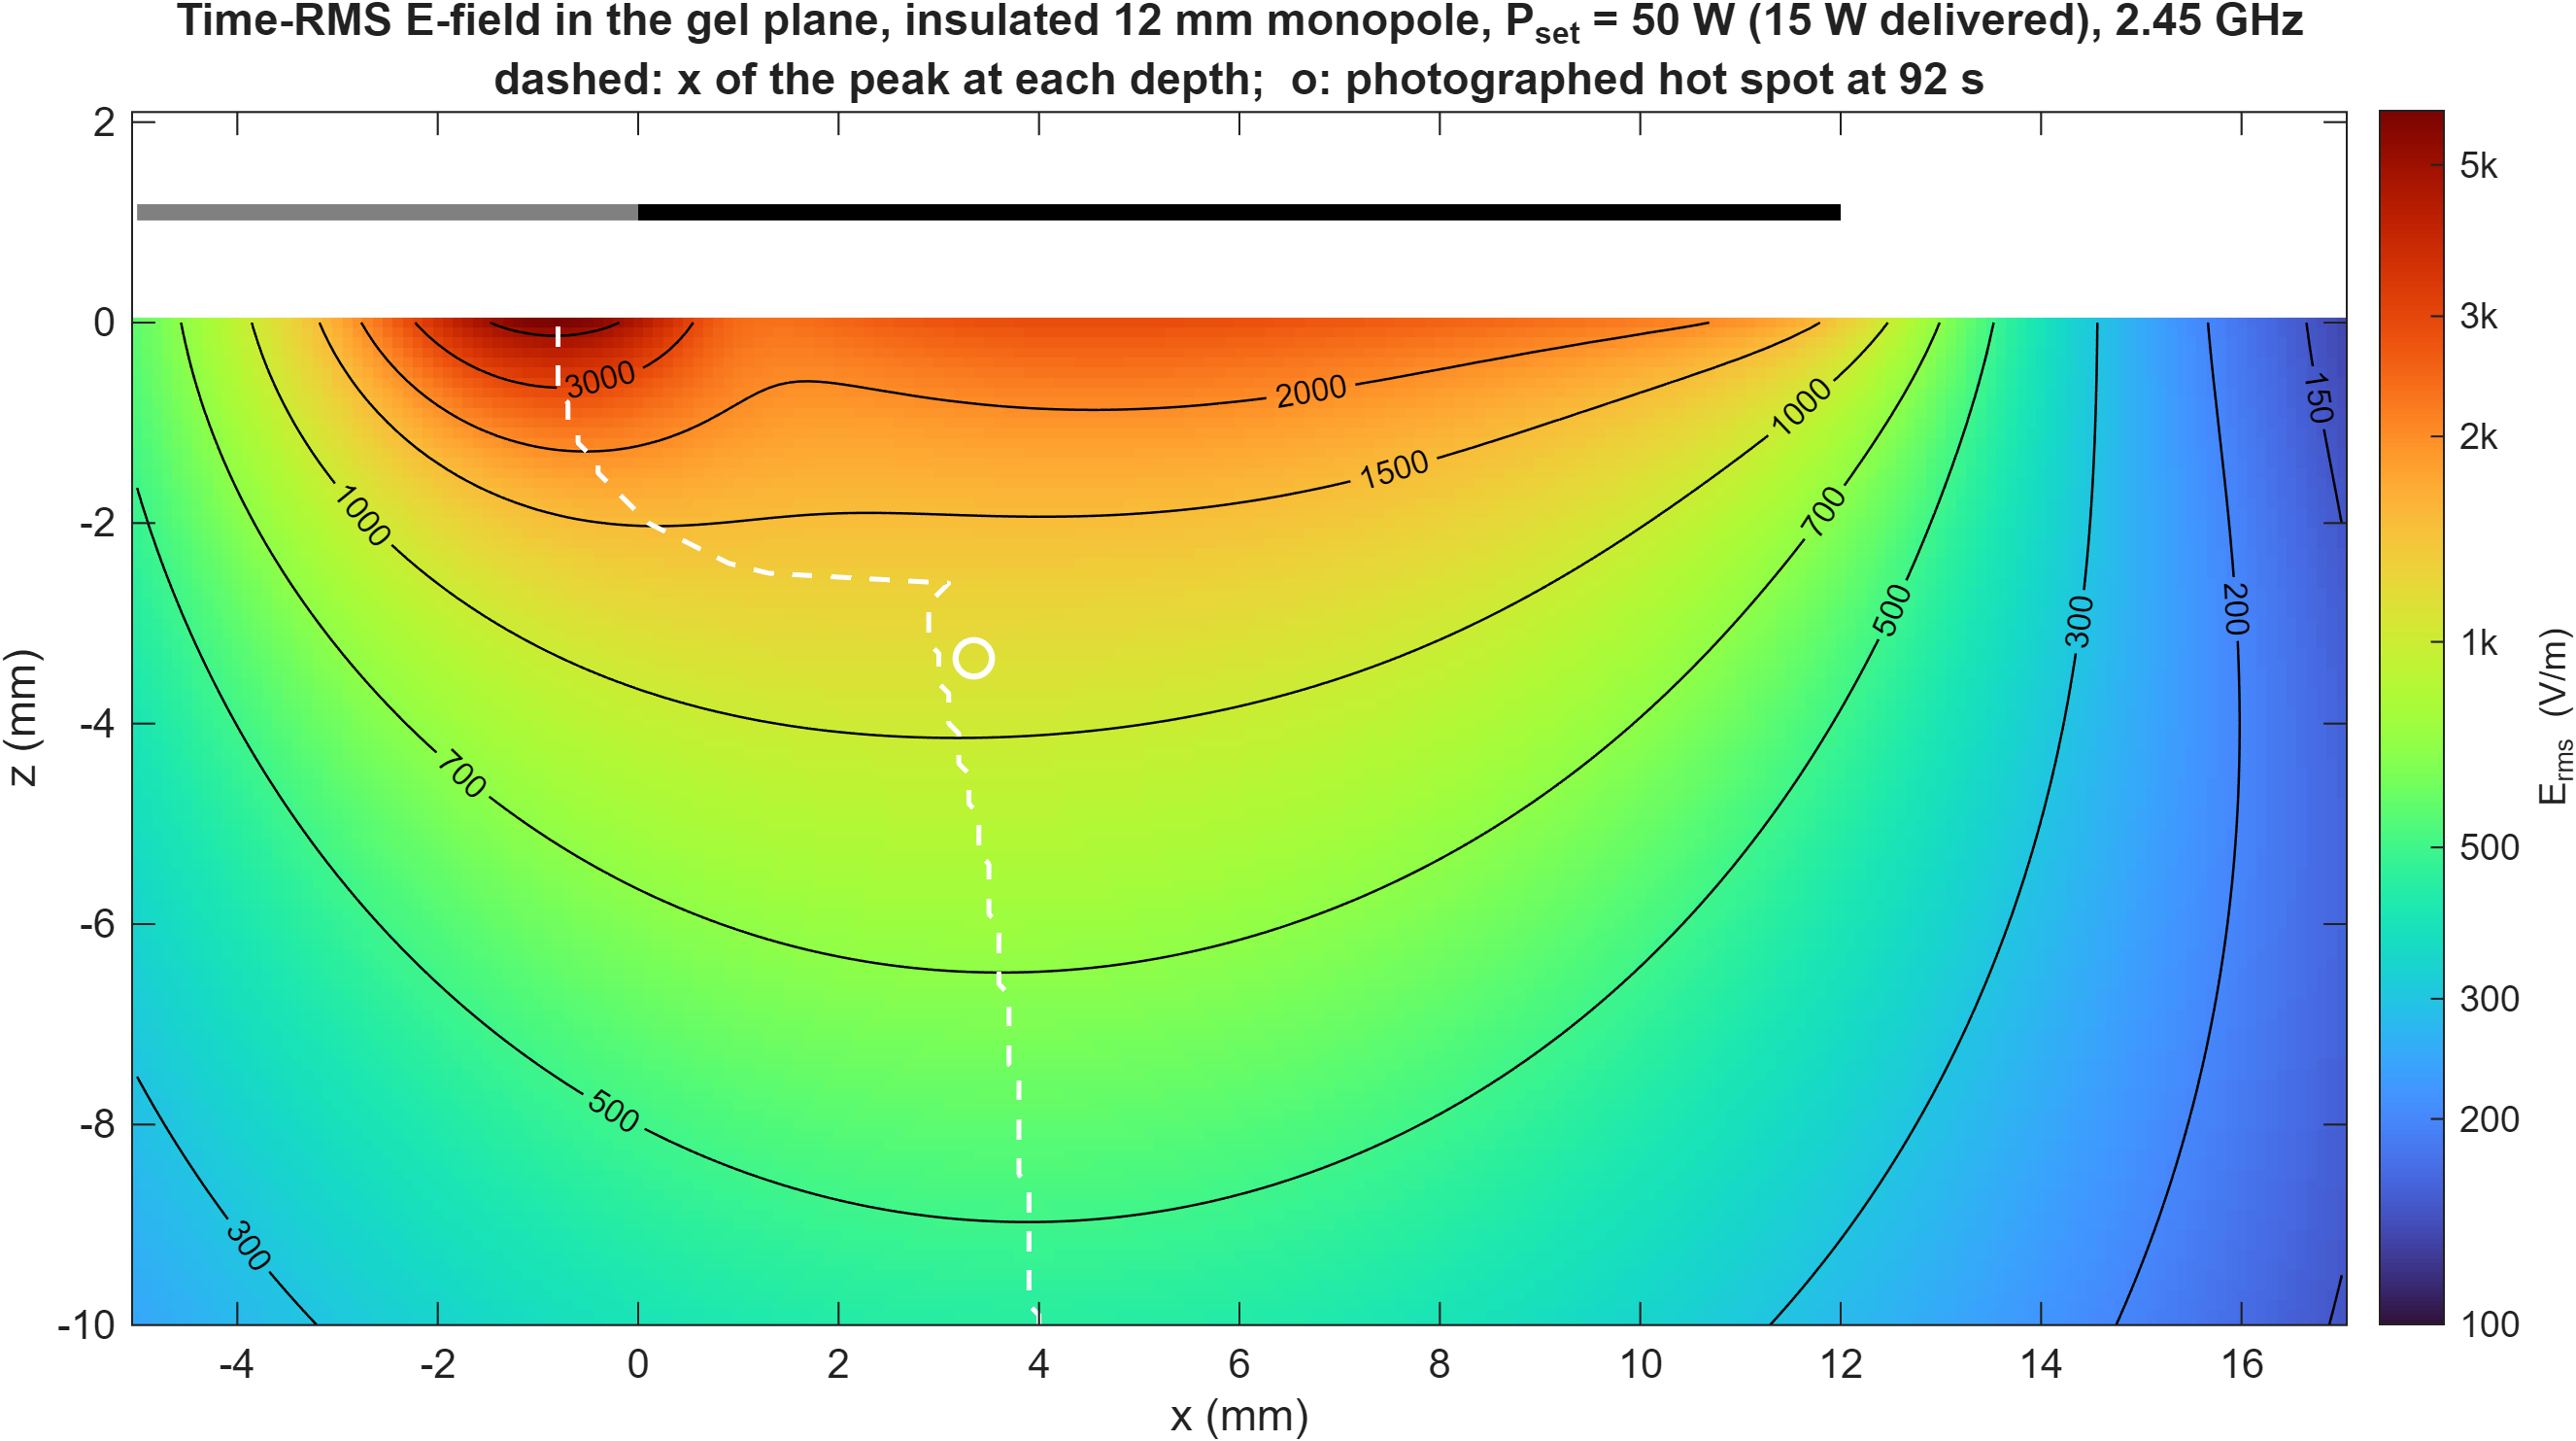
\includegraphics[width=\textwidth]{Erms_insulated_monopole.png}
  \caption{$\Erms$ in the gel plane below the antenna, as produced by the script. Grey: feed cable. Black:
  12\,mm insulated element. The dashed line tracks the $x$ position of the peak at each depth. The circle
  marks the hot spot in the photograph at 92\,s.}
  \label{fig:map}
\end{figure}

The script reports $k_L=126.0-29.7\jj$\,rad/m, $Z_{\text{in}}=23.9-9.6\jj\,\Omega$ and $I_0=1.12$\,A. The
field map (Fig.~\ref{fig:map}) has two regimes.

At the gel surface the strongest field, 5.9\,kV/m, sits at $x=-0.8$\,mm, directly under the feed block.
Splitting \eqref{eq:Ex}--\eqref{eq:Erho} into their terms shows that this peak is almost entirely the
vertical charge field $E_\rho$ from the packed block charge of \eqref{eq:block}: about 5.6\,kV/m, against
2.0\,kV/m from the current term. At 1\,mm depth the peak is still behind the feed (2.3\,kV/m at
$x=-0.7$\,mm). By 2\,mm it has moved to the feed ($1.5$\,kV/m at $x=0.1$\,mm). The field of this charge
concentration decays quickly with depth. In the experiment it also sits in the top $\sim$2\,mm of gel, where
the circulating water holds the surface near the water temperature. That is consistent with the absence of a
visible hot spot there in the photographs.

Below about 2.5\,mm the peak jumps forward and stays 3--4\,mm in front of the feed: 1.2\,kV/m at
$x=2.9$\,mm and 3\,mm depth, 0.87\,kV/m at $x=3.4$\,mm and 5\,mm depth, and 0.44\,kV/m at $x=4.0$\,mm and
10\,mm depth. In this regime the inductive current term dominates. At 3\,mm depth it is about 1.5\,kV/m, and
the charge term (about 0.45\,kV/m) partly cancels it. The forward shift is a geometric effect of the current
distribution. A point at depth $D$ averages the current over a window of the element roughly $D$ wide,
because the kernel $G(R)$ weights nearby sources most. Under the feed, half of that window lies behind the
feed, where only the short block carries current, so the average is low. Moving forward fills the window,
but the quarter-wave current \eqref{eq:Ielem} falls toward the tip. The product of these two effects peaks
a few millimetres in front of the feed.

The photographed hot spot at 92\,s sits at $(x,z)\approx(3.35,-3.35)$\,mm, on the dashed peak track in
Fig.~\ref{fig:map}. The photographs show the hot spot 2--4\,mm in front of the feed at 2.5--4.5\,mm depth
over the run. A separate three-dimensional conduction calculation in this project, driven by this field
with the gel surface held at the water temperature, placed the thermal peak at
$(3.0, 2.25)$, $(3.25, 3.0)$ and $(3.5, 4.25)$\,mm ($x$, depth) at 29, 92 and 332\,s, in agreement with the
photographs.

\section{Summary of assumptions}\label{sec:assumptions}

The assumptions introduced above are collected here in the order they enter the calculation.

The inputs are taken from two sources. The geometry comes from the photograph and the RG-178 datasheet, not
from the setup table, because the photographed antenna is 12\,mm long with the PTFE left on. The water is
treated as pure (non-saline). PTFE loss is neglected. The delivered power is the generator setting times
the estimated factor $1-P_{\text{dropoff}}$, and no power is reflected.

The current wavenumber relies on King's conditions $|k_w/k_{\text{ins}}|^2\gg1$, $|k_{\text{ins}}b|^2\ll1$ and
$|k_wb|<1$, all of which are satisfied. The antenna is modelled as a single open-circuited arm of insulated
line, with the fringing capacitance at the tip neglected. The return current is confined to the 1.5\,mm feed
block with a linear profile, and there is no sheath current on the braid. This last choice has the greatest
influence on where the peak falls.

The field calculation uses thin-wire filament sources. It treats the gel as a homogeneous half-space and
uses the gel Green's function throughout. The water--gel interface enters only through the quasi-static
transmission factor $\tau$, applied to the charge term. Reflected and lateral waves at the interface, the
finite size of the gel block, and the slight violation of the Lorenz condition that $\tau$ introduces are
all neglected.

Finally, the conversion to heating uses $\sigma_{\text{eff}}=\omega\eps_0\eps_g''$. This value differs from
the 1.7\,S/m conductivity quoted in the setup table.

\begin{thebibliography}{99}

\bibitem{King1983}
R.~W.~P. King, B.~S. Trembly and J.~W. Strohbehn,
``The electromagnetic field of an insulated antenna in a conducting or dielectric medium,''
\emph{IEEE Transactions on Microwave Theory and Techniques}, vol.~31, no.~7, pp.~574--583, 1983.

\bibitem{KingSmith1981}
R.~W.~P. King and G.~S. Smith,
\emph{Antennas in Matter: Fundamentals, Theory, and Applications}.
Cambridge, MA: MIT Press, 1981.

\bibitem{Jackson1999}
J.~D. Jackson, \emph{Classical Electrodynamics}, 3rd~ed. New York: Wiley, 1999.
(\S4.4, boundary-value problems with dielectrics; \S6.2--6.4, potentials, Lorenz gauge and the retarded
Green's function.)

\bibitem{Balanis2016}
C.~A. Balanis, \emph{Antenna Theory: Analysis and Design}, 4th~ed. Hoboken, NJ: Wiley, 2016.
(Chs.~3--4, radiation integrals and thin linear wire antennas.)

\bibitem{Pozar2012}
D.~M. Pozar, \emph{Microwave Engineering}, 4th~ed. Hoboken, NJ: Wiley, 2012.
(Ch.~2, telegrapher's equations, terminated lossy lines and power flow.)

\bibitem{Harrington1961}
R.~F. Harrington, \emph{Time-Harmonic Electromagnetic Fields}. New York: McGraw-Hill, 1961.
(Ch.~1, phasors, complex permittivity and time averages.)

\bibitem{AbramowitzStegun1964}
M. Abramowitz and I.~A. Stegun (eds.), \emph{Handbook of Mathematical Functions}. Washington, DC: National
Bureau of Standards, 1964. (\S9.1, small-argument forms of Bessel and Hankel functions.)

\bibitem{vonHippel1954}
A.~R. von Hippel (ed.), \emph{Dielectric Materials and Applications}. Cambridge, MA: MIT Press, 1954.

\bibitem{Kaatze1989}
U. Kaatze, ``Complex permittivity of water as a function of frequency and temperature,''
\emph{Journal of Chemical and Engineering Data}, vol.~34, no.~4, pp.~371--374, 1989.

\bibitem{MIL17}
MIL-DTL-17/93, \emph{Cables, radio frequency, flexible, coaxial, 50 ohms, M17/93-RG178}.
U.S. Department of Defense specification sheet.

\bibitem{KingOwensWu1992}
R.~W.~P. King, M. Owens and T.~T. Wu,
\emph{Lateral Electromagnetic Waves: Theory and Applications to Communications, Geophysical Exploration,
and Remote Sensing}. New York: Springer, 1992.

\end{thebibliography}

\end{document}
